\section{GPA Embeddings}\label{sec:methods}

The defining relations for $\DD_3$ and $\DD_4$ were not computed theoretically. Instead, we deduced them from embedding the planar algebras $\PP_{Y_4;\cat{q_3}_{A_3}}$ and $\PP_{Y_4;\cat{q_4}_{A_4}}$ into graph planar algebras.

One may give a functor $F:\GG_2(q_k) \to \GPA(\Gamma)$ by giving the image of the morphism 
\[
F\left( \skein{skein_figs/trivalent}{0.08} \right) \in \Hom_{\GPA(\Gamma)}(2\to1).
\]
This amounts to giving a list of $M\coloneqq\tr(\Gamma^2\cdot\Gamma)$ complex scalars\footnote{
    We freely switch between using $\Gamma$ to mean the graph itself and the graph's adjacency matrix. }, 
say $a_1,\dots,a_M$. These complex numbers satisfy equations in the $a_i$ and $\ol{a_i}$. If we assume for now that each $a_i$ is real, then this reduces the system to a collection of polynomials in the $a_i$ \footnote{This assumption is useful only if it turns out to help us solve the system. In fact, any assumptions we make about this system, if they yield solutions, are in some way valid.}.
Once we have the image of the trivalent vertex in hand, we have found an embedding of the planar algebra it generates. We can then solve for the image
\[
F\left( \skein{skein_figs/Pg}{0.08} \right) \in \Hom_{\GPA(\Gamma)}(2\to2)
\]
to extend the GPA embedding of $\GG_2(q_k)$ to an embedding of $\DD_k$.

\subsection{Trivalent Vertex}\label{subsec:triv-vertex}


\begin{figure}
    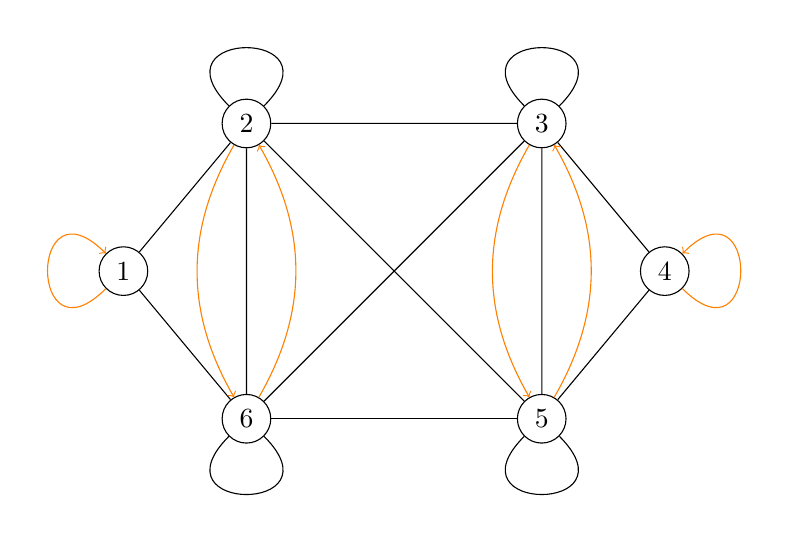
\begin{tikzpicture}[scale=1.25]
        \node[shape=circle,draw=black] (A) at (0,1.5) {1};
        \node[shape=circle,draw=black] (B) at (1.25,3) {2};
        \node[shape=circle,draw=black] (C) at (4.25,3) {3};
        \node[shape=circle,draw=black] (D) at (5.5,1.5) {4};
        \node[shape=circle,draw=black] (E) at (4.25,0) {5};
        \node[shape=circle,draw=black] (F) at (1.25,0) {6};

        % module fusion graph
        \path (B) edge [loop, in=45, out=135, looseness=8] node {} (B);
        \path (C) edge [loop, in=45, out=135, looseness=8] node {} (C);
        \path (E) edge [loop, in=225, out=315, looseness=8] node {} (E);
        \path (F) edge [loop, in=225, out=315, looseness=8] node {} (F);

        \path [-] (A) edge node {} (B);
        \path [-] (A) edge node {} (F);

        \path [-] (B) edge node {} (C);
        \path [-] (B) edge node {} (E);
        \path [-] (B) edge node {} (F);

        \path [-] (C) edge node {} (D);
        \path [-] (C) edge node {} (E);
        \path [-] (C) edge node {} (F);

        \path [-] (D) edge node {} (E);

        \path [-] (E) edge node {} (F);

        % g fusion graph
        \path [->, draw=orange] (A) edge [loop, in=135, out=225, looseness=8] node {} (A);
        \path [->, draw=orange] (D) edge [loop, in=45, out=-45, looseness=8] node {} (D);

        \path [->, draw=orange] (B) edge [bend right] node  {} (F);
        \path [->, draw=orange] (F) edge [bend right] node {} (B);

        \path [->, draw=orange] (C) edge [bend right] node {} (E);
        \path [->, draw=orange] (E) edge [bend right] node {} (C);
    \end{tikzpicture}
    \caption{Fusion graphs at level 4 for $Y$ (black) and $g$ (orange). See \cite[Figure 21b]{g2_graphs}.}
    \label{fig:new-graphs-lvl4}
\end{figure}



The goal of this subsection is to describe in more detail the process of finding the image of the trivalent vertex. 
We will walk through the details for the level 4 case. 
The level 3 case follows the same process, but is less computationally instructive.
However, the level 3 case does offer some insights into the relationship between embedding coordinates 
and symmetries of the funamental graph. 
In Subsection~\ref{subsec:results-3} we will explore this relationship further.
Figure~\ref{fig:new-graphs-lvl4} shows the module fusion graph at level 4.

Let 
\[
    (p_1,q_1),\dots,(p_M,q_M)
    \footnote{ See the attached Mathematica files for the specific ordering chosen. }
\]
be the defining basis for $\Hom_{\GPA(\Gamma)}(2\to1)$ ($M=88$ at level 4). Then it must be that 
\[
    F\left( \skein{skein_figs/trivalent}{0.08} \right) = a_1(p_1,q_1)+\cdots+ a_M(p_M,q_M).
\]
The \ref{eq:Bigon} relation, when sent through $F$, becomes the system
\[
    \sum_{i=1}^M a_i(p_i,q_i) \circ \sum_{j=1}^M a_j(q_j,p_j) = k^2 \sum_{e\in E(\Gamma)} (e,e).
\]
This system is quadratic in the $a_i$ since it involves up to two trivalent vertices on either side. The \ref{eq:Lolli} and \ref{eq:Rotate} relations therefore determine a system of linear equations; the others give cubic, quartic, and quintic equations. It is often useful to solve the linear subsystem first and substitute the solution into the quadratic equations. For example, at level 4, discussed in Section~\ref{sec:level-4}, we solve the linear subsyetm, substitute the solution, and isolate the following resulting equations:
\begin{align*}
    a_{8}^2+a_{85}^2 & = 4-\sqrt{2}+2 \sqrt{3}-\sqrt{6} \\
    a_{69}^2+\left(1+\sqrt{\frac{3}{2}}\right) a_{8}^2 & = \frac{3+\sqrt{3}+\sqrt{6}}{\sqrt{2}} \\
    a_{69}^2 \left(\left(2+\sqrt{6}\right) a_{8}^2+\left(2+\sqrt{6}\right)
   a_{85}^2-2 \sqrt{2+\sqrt{3}}\right) & = 5+\sqrt{2}+\sqrt{3}+2 \sqrt{6} \\ 
   2 a_{69}^4+\left(5+2 \sqrt{6}\right)
   a_{85}^4 & = \left(3+\sqrt{2}+\sqrt{3}+\sqrt{6}\right) a_{85}^2+3
   \sqrt{6}+\sqrt{3}+2 \sqrt{2}+7 \\
\end{align*}
Up to three choices of sign, the solution to this system is
\begin{align*}
    a_{8} & = \sqrt{2+\sqrt{3}-\sqrt{2+\sqrt{3}}} \\
    a_{69} & = \sqrt{\frac{1}{2} \left(-1+\sqrt{2}+\sqrt{3}\right)} \\
    a_{85} & = \sqrt{2+\sqrt{3}-\sqrt{2+\sqrt{3}}} \\
\end{align*}
Similar equations containing $a_{31}$, $a_{55}$, and $a_{63}$ appear as well. We may repeat this process and obtain the additional values
\begin{align*}
    a_{31} & = \sqrt{2+\sqrt{3}-\sqrt{2+\sqrt{3}}} \\
    a_{55} & = \sqrt{1-\sqrt{\frac{3}{2}}+\frac{1}{\sqrt{2}}} \\
    a_{63} & = \sqrt{2+\sqrt{3}-\sqrt{2+\sqrt{3}}} \\
\end{align*}
These six degree-8 algebraic numbers now begin a cascade of equation solving. They, along with the linear solution, reduce many of the original high-order equations to linear. We solve those, then repeat the process until we're forced to confront nonlinearity. The nonlinearity we encounter forces us to extract square roots, and ending up with degree-16 algebraic numbers. This lead to us concluding, for instance, that
\[
    a_{10} = \frac{1}{2} \left(\sqrt{1+\sqrt{6-3 \sqrt{3}}}+\sqrt{\sqrt{2+\sqrt{3}}-1}\right).
\]




\subsection{Projection and its relations}\label{subsec:proj-relns}
The process of finding a GPA embedding of the projection 
$\skein{/skein_figs/Pg}{0.08}$ is similar to the process of finding the trivalent vertex described above. 
Now, however, we must use relations involving both 
$\skein{/skein_figs/trivalent}{0.08}$ and $\skein{/skein_figs/Pg}{0.08}$. 
Call the coordinates of the projection $b_i$. 
Since the coordinates of the trivalent vertex are now known, 
the degree of the resulting equations now depends only on the number of projection strands appearing.
Moreover, we do not necessarily assume the $b_i$ are real; 
hence the resulting equations are polynomial in $b_i$ and $\ol{b_i}$. 

The relation (decStick) along with the one-strand relations of (Schur 0) and (Schur 1) give a system of linear equations. 
The following proposition, which is a specialization of Proposition~\ref{prop:hb-general} 
to the case where $f=P_g$, provides an additional set of linear equations in the projection coefficients.

\begin{proposition}
    The following relation holds:
    \begin{equation*}\tag{Half-braid}
        \skein{/skein_figs/hb_top}{0.15} = \skein{/skein_figs/hb_bottom}{0.2}
    \end{equation*}
\end{proposition}

The relation (Half-braid) is not used in the evaluation algorithm.
It is merely a vehicle for obtaining a huge set of linear equations in the $b_i$ and $\ol{b_i}$.

In total, the linear system was enough to fully determine the projection coefficients for both levels 3 and 4.
It is at this point that the present work diverges from other similar published works on the topics of
GPA embeddings \cite{Cain_Dan} or presentations for conformal embeddigns \cite{cain_noah}.
Previous investigations utilizing GPA embeddings have had a full set of relations on hand,
and these relations were used to {\it find} the embeddings.
On the other hand, recent progress on conformal embeddings have used theoretical means to uncover relations.

At the present step in this work, we are standing before an unexplored category, with an embedding 
of two of its generators, $\skein{/skein_figs/trivalent}{0.1}$ and $\skein{/skein_figs/Pg}{0.1}$, in hand.
We have a set of relations for $\skein{/skein_figs/trivalent}{0.1}$ 
(i.e., the defining relations of $\GG_2(q)$) sufficient to evaluate any undecorated closed diagram.
However, we do not know what further relations we will find, nor exactly when we ought to stop looking.
% When searching for a GPA embedding of the underlying trivalent category, 
% we had a set of known relations on the trivalent vertex; i.e., the defining relations of $\GG_2(q)$. 
In order to uncover relations such as those of Definition~\ref{def:zn-ext}, 
we use a process reminiscent of the scientific method. 
This process begins by considering a decorated trivalent diagram and searching for ways to decrease its complexity. 
We begin the process by assuming no more than a minimal collection of moves; i.e., (decStick), (Recouple), and ($\Z_n$).
Once we have applied all these minimal moves, we begin to look for 
a move we might hope to make, and assume it comes at some cost. 
For example, being able to apply (Swap) might allow us to then apply (decStick); 
thus we would eliminate a colored strand at the cost of a scalar $\omega$. 
This is clearly a trade we should make.
In order to find the exact price of this trade, we use our GPA-embedding $F:\DD_3 \to\GPA(\Gamma_3)$, 
and assume we know the form the cost will come in.
We use the embedding coefficients we previously found to set up and solve the linear equation
\[
    F\left( \skein{/skein_figs/swap_LHS}{0.15} \right) = \omega F\left( \skein{/skein_figs/swap_RHS}{0.15} \right)
\]
for $\omega$.

Another example of this tradeoff appears in the proof of Lemma~\ref{lem:ext-dec}. 
During the proof, we apply (Swap) and (Change of Basis) with the goal of ridding ourselves of internal strands; 
this comes at the cost of external strands.
The costs incurred in the (decTrigon), (decTetragon), and (decPentagon) relations are less straightforward to predict.
The form the relations are presented in is the product of trial and error. 
As one will note when inspecting the coefficients of these relations in the attached Mathematica files,
many of the (decTetragon) and (decPentagon) coefficients are zero.
The obvious next question one asks is which of the numbers $u_{i,j}$, $v_{i,j}$, and $w_{i,j}$ one should expect to be nonzero.
The examples we construct based on $\GG_2(q)$ are too isolated to notice a pattern and draw conclusions in general.
However, forthcoming work of the present author and Edie-Michell constructing many 
examples of near-groups as $Z_n$-like extensions will work to shed light on the phenomenon as a whole.
